\documentclass[10pt]{article}         %% What type of document you're writing.

%%%%% Preamble

%% Packages to use
\usepackage{amsmath,amsfonts,amssymb,graphicx}   %% AMS mathematics macros
\usepackage[german]{babel}
\usepackage[utf8]{inputenc}
\usepackage{titlesec}
\usepackage{courier}
\usepackage{textcomp}
\usepackage[procnames]{listings}
\usepackage{color}

\setcounter{secnumdepth}{4}
\titleformat{\paragraph}
{\normalfont\normalsize\bfseries}{\theparagraph}{1em}{}
\titlespacing*{\paragraph}
{0pt}{3.25ex plus 1ex minus 0.2ex}{1.5ex plus 0.2ex}


%% Title Information.
\title{Optimierungsmethoden}
\author{Timon Tschanz, Pascal Zingg}
%% \date{}           %% By default, LaTeX uses the current date

%%%%% The Document

\begin{document}

\definecolor{keywords}{RGB}{131,0,90}
\definecolor{comments}{RGB}{88,88,88}
\definecolor{blue}{RGB}{17,51,160}
\definecolor{green}{RGB}{0,120,0}


\lstset{basicstyle=\footnotesize\ttfamily,
    commentstyle=\color{Gray}\ttfamily,
    belowcaptionskip=5em,
    belowskip=4em,
}

\maketitle

\section{Einführung}
Im Rahmen des Kurses Analysis haben wir uns mit verschiednen Optimierungsaufgaben vertraut gemacht. Die grundlegende Technik, die wir dazu verwendeten, war die 1. Ableitung gleich 0 zu setzen, damit wir ein optimales Ergebnis für ein konkretes Problem erhielten. In diesem Bericht befassen wir uns näher mit Algorithmen, welche es ermöglichen Extremalstellen zu berechnen. Zudem diskutieren wir anhand von diversen Aufgabenstellungen, wie diese zur Anwendung kommen können. Durch diverse Visualisierungen versuchen wir mit diesem Bericht versuchen wir die Ergebnisse bildlich darzustellen, was aus unserer Sicht auch zu einer glaubwürdigeren Diskussion führen wird und die Probleme gut veranschaulichen lassen.

\section{Motivation}
Da es in unserer Umgebung sehr viele Problemstellungen gibt, bei denen jeweils ein Optimum gesucht ist, sehen wir in dieser Arbeit eine konkrete und relativ einfache Anwendung der Ableitungen. Die Algorithmen, welche wir mit Python umgsetzt haben, sind wiederverwendbar, da wir sie so weit als möglich versuchten, zu parametrisieren. 

\pagebreak
\section{Auswertungsverfahren}
\subsection{Algorithmen}
Um die Extremalstellen einer spezifischen Funktion zu errechnen, gibt es diverse Vorgehensweisen. In diesem Kapitel gehen wir auf die 3 im Unterricht behandelten Verfahren ein und erläutern ihre Funktionsweise. 

\subsubsection{Gradientenverfahren}
Durch diese Methode wird im generellen versucht, sich an eine Extremalstelle anzunähren. $x_0$ wird als Startpunkt definiert. Vorausgesetzt wird hierbei, dass sich der Punkt links von einer Extremalstelle befindet. Veranschaulichen wir uns die nachfolgende quadratische Funktion:
\[
    f(x)=x^2
\]

Abbildung~\ref{gradientx} verdeutlicht anhand der quadratischen Funtkion das `Abtasten' und Annähern an eine Extremalstelle. Durch das festgesetzte Lambda wird das Offset für die verschiedenen Punkte festgesetzt. Dies hat je nach Konfiguration dieses Parameters Konsequenzen auf die Laufzeit unseres Algorithmus. Im nachfolgenden Abschnitt werden wir versuchen, Lambda sinnvoll zu bestimmen.

\begin{figure}[!ht]
    \centering
    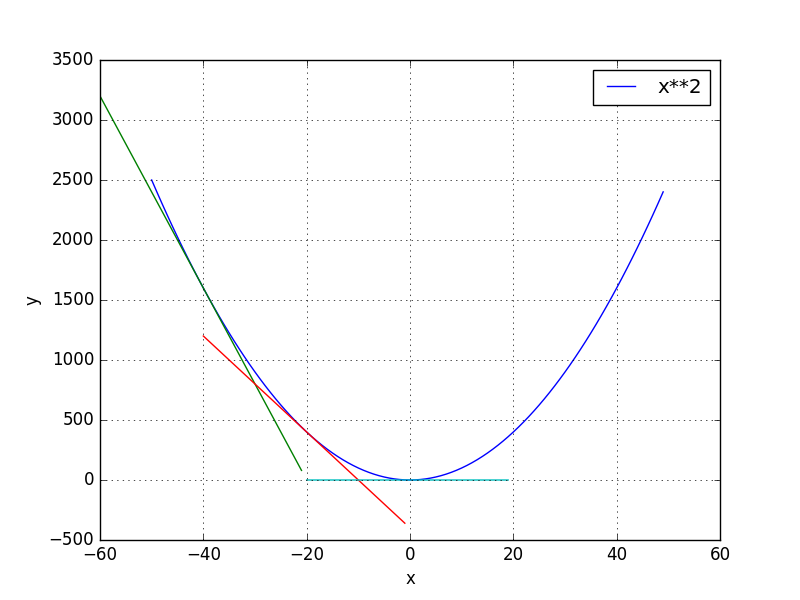
\includegraphics[width=0.9\textwidth]{gradient}
    \caption{Funktion $x^2$ mit Annäherung an Extremalstelle}\label{gradientx}
\end{figure}

\paragraph{Laufzeit}
Da die Laufzeit von der Entfernung abhängt, welche zwischen dem gewählten Punkt und der Extremalstelle definiert ist, und wir des weiteren auch Lambda als Parameter berücksichtigen müssten, ist es uns nicht gelungen, die Laufzeit in der Big-O Notation auszudrücken.

Dafür implementierten wir für diesen Algorithmus eine Schlaufe, welche mit unterschiedlichen Lambdas die Zeit misst. Dies setzten wir anhand der obigen Funktion $x^2$ um. Folgende Messwerte erhalten wir:\\

\lstinputlisting[language=bash]{grad_time.out}


Die obigen Berechnungen wurden mit der quadratischen Funktion $x**2$ durchgeführt und als Anfangspunkt wurde $x=-5$ gwählt. Dieser hat jedoch keinen Einfluss, da die Berechnungen immer relativ zueinander stehen. 
Wie wir aus dem Output entnehmen können, sind sowohl $0.0001$ wie auch $1$ nicht sinnvoll für die Verwendung von Lambda. Zum Einen ist bei der Wahl eines kleinen Wertes für Lambda die Laufzeit stark negativ beeinträchtigt. Jedoch ist das Resultat sehr genau. Wählen wir eine grössere Zahl für Lamdba, so ist ersichtlich, dass die Genauigkeit nicht mehr gewährleistet ist, da der Algorithmus in grösseren Schriten sich an die Nullstelle annähert. 

\paragraph{Bedingungen}
In Abbildung~\ref{gradientx} wird veranschaulicht, wie der Algorithmus funktioniert. Als Vorbedingung ist ein Startpunkt notwenig, welcher zwingend links von einer Extremalstelle liegt. Ausserdem muss mit diesem trivialen Algorithmus vorher sichergestellt werden, dass die Funktion überhaupt Extremalstellen besitzt, was ansosten zu einem unendlichen Loop führen kann. Des Weiteren sagt das Vorzeichen von Lambda aus, nach welcher Art von Extremstelle gesucht werden soll. In unserem Beispiel mit der quadratischen Funktion $x^2$ wählen wir zum Beispiel den Punkt $x=-5$ aus. Wir können uns versichern, dass der Punkt links von einer Extremalstelle (links) liegt und die Funktion überhaupt eine Extremalstelle besitzt. Natürlich ist diese von blossem Auge sofort erkennbar. 
Wir fassen zusammen:
\begin{itemize}
\item Punkt muss links von Extremalstelle liegen
\item Typ von gesuchter Extremalstelle muss bekannt sein (Minimum oder Maximum)
\item Lambda wird wie folgt gewählt: $Lambda > 0 = Minimumsuche, Lambda > 0 = Maximumsuche$
\end{itemize}

\paragraph{Funktion von Lambda}
Der Algorithmus beginnt also vom Punkt $x=-5$ an, die 1. Ableitung zu berechnen. Hat er diese berechnet und ist diese ungleich 0, so wird mit Lambda ein neuer Punkt definiert, welcher sich etwas weiter Rechts auf der x-Achse befindet. Der Algorithmus ist so aufgebaut, dass er eine gewisse Genauigkeit aufweisen muss, um eine Extremalstelle eindeutig zu identifizieren. Diese Genauigkeit muss unbedingt kleiner sein als Lambda, da sonst die Stelle einfach übersprungen werden kann.

\subsubsection{Nelder-Mead}
Der Nelder-Mead Algrithmus versucht basierend auf zwei original gegebenen Punkten ein Extrema zu finden. Er erreicht das Ziel in dem er basierend auf den originalen Punkten weitere Punkte generiert und analysiert, ob die Punkte kleiner (respektive grösser) sind und ruft sich dann erneut auf mit einem der extremeren Punkten. Aufgrund dieser Funktionsart findet der Nelder-Mead entweder Maximas oder Minimas aber nicht beide zusammen. Da bei der Versicherungsaufgabe der Gewinn gesucht wird, haben wir den Nelder-Mead auf die Suche von Maximas ausgelegt.

\paragraph{Laufzeit}
Der Algorithmus läuft im schlechtesten Fall in $O(n^2)$ $^1$

\paragraph{Bedingungen}
Da der Nelder-Mead sich auch Punkte ausserhalb der angegebenen Punkte sucht, muss die Funktion auch ausserhalb dieser Punkte definiert sein oder allenfalls so konstruiert werden, dass diese Punkte nicht in Betracht gezogen werden.

\subsubsection{Nullstelle der Ableitung}
Durch den Bisektionsalgorithmus kann mithilfe der Ableitung eine Nullstelle, dass heisst eine Extremalstelle ermittelt werden. Durch den Gebrauch eines anderen Algorithmus, in unserem Falle der Bisektionsalgorithmus, näheren wir uns ähnlich wie mit dem Gradientenverfahren an die Nullstelle an. 

\begin{figure}[!ht]
    \centering
    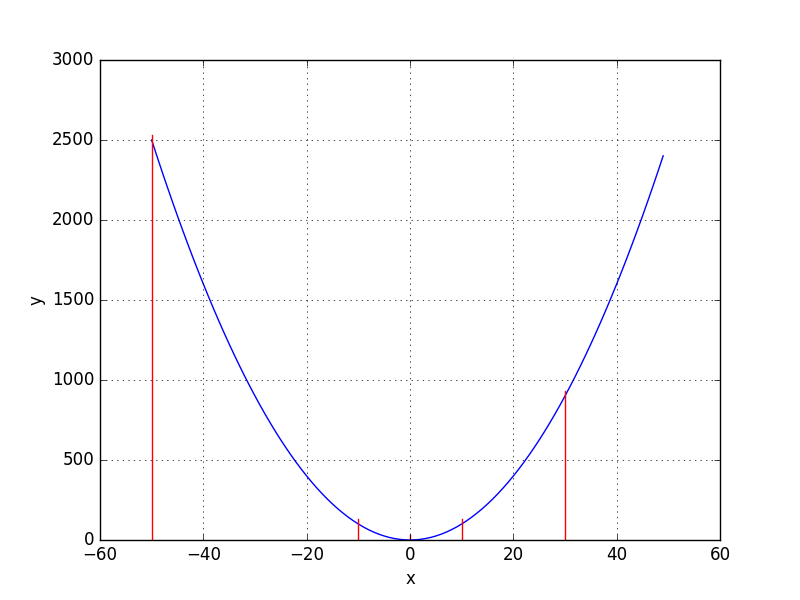
\includegraphics[width=0.9\textwidth]{bisektion}
    \caption{Bisektionsalgorithmus}\label{bisektion}
\end{figure}

Wie der Abbildung~\ref{bisektion} entnommen werden kann, schränkt sich der Bereich einr möglichen Nullstelle durch eine linke und rechte Schranke immer mehr ein.

\paragraph{Laufzeit}
Da der Bisektionsalgorithmus immer halbiert wird, das heisst die durchzusuchenden Wertebereiche logarithmisch schrumpfen, wird die Laufzeit vom Intervall $n=b-a$ gleich $O(\log(n))$ betragen. Die Berechnung der Ableitung wird hier wie bei den anderen Methoden ausser Acht gelassen. Wir können hierbei also feststellen, dass der Algorithmus effizient ist. Leider trübt dieser Vorteil, da er doch sehr eingeschränkt verwendet werden muss, was im nächsten Abschnitt näher erläutert wird.

\paragraph{Bedingungen}
Es muss vorgänig ein Intervall definiert werden, in welchem Extremalstellen anzutreffen sind. Unglücklicherweise kann bei zwei solchen Stellen nicht differenziert werden, dass sich tatsälich mehrere Stellen in dem Intervall befinden. Aus diesem Grund muss für unseren Algorithmus folgende Vorbedingung erfüllt werden: Der Intervall, welcher im Voraus definiert wird, darf nur genau eine Extremalstelle beinhalten. Wir haben uns Gedanken gemacht, wie wir dieses durchaus unschöne Problem lösen könnten. Man dürfte keine der ignorierten Seiten des Bisektionsalgorithmus ausser Acht lassen, da sich dort weitere Stellen befinden könnten. Dies würde den grundsätzlichen Nutzen des Bisektionsalgorithmus zerstören. Aus diesem Grund beschlossen wir, die Vorbedingung wie bereits erwähnt aufzustellen.

\pagebreak
\section{Anwendungsbeispiele}
\subsection{Der Rettungsschwimmer}
Ein Rettungsschwimmer will einer ertrinkenden Person im Wasser helfen. An Land rennt er mit $4.1 m/s$, im Wasser schwimmt er mit $2.1 m/s$. Welcher Weg an Land und im Wasser ist optimal, um in möglichst geringer Zeit zum Ertrinkenden zu gelangen? \\
    Diese Aufgabe klingt an sich trivial. Ein kleines Hindernis gibt es hierbei aber: Es sind keine Längenangaben vorhanden, was bedeutet, dass wir ein parametriesertes Ergebnis erwarten müssen. Abbildung~\ref{retts} zeigt, wie wir die Längen aufgeteilt haben.

\begin{figure}[!ht]
    \centering
    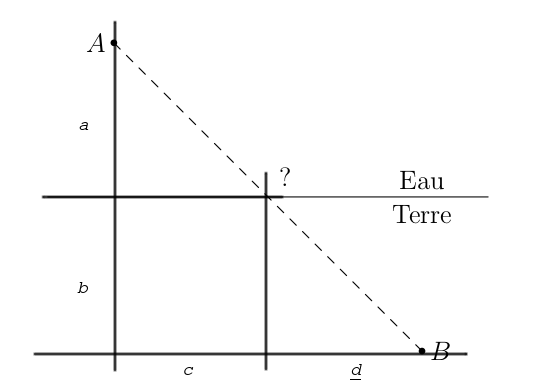
\includegraphics[width=0.9\textwidth]{rettungsschwimmer}
    \caption{Rettungsschwimmer}\label{retts}
\end{figure}

Da keine Längenangaben vorhanden sind, versuchten wir mittels verschiedenen Annahmen, uns an eine mögliche allgemeine Lösung für das Problem heranzutasten. Wie in~\ref{retts} eingezeichnet, gibt es die vier variablen Längen $a, b, c, d$. Kümmern wir uns zuerst um das Aufstellen einer Gleichung für das Optimierungsproblem. Uns ist bekannt, dass sich die Geschwindigkeit $v$ aus $s/t$ zusammensetzt. Des weiteren Wissen wir, nach was wir Optmimieren müssen: Der Zeit $t$. \\
Nach Pythagoras können wir auch die Längen berechnen, welche sich aus den Teilstrecken ergeben:
\begin{align}
    s_1=\sqrt{a^2+c^2} \\
    s_2=\sqrt{b^2+d^2}
\end{align}

Uns liegt nun auch auf der Hand, wie wir die Gleichung aufstellen müssen, um nach der Zeit zu optimieren. Allgemein lassen sich Optimierungsprobleme lösen, in dem die Ableitung der Gleichung gleich 0 gesetzt wird und nach einer gewünschten Variable aufgelöst wird. Wir beginnen zunächst, die Gleichung zusammenzusetzen. Um die optimale Zeit zu erhalten, müssen wir versuchen, die Summe der Zeit während des Laufens und die Zeit wärend des Schwimmens in Form einer Gleichung darzustellen. Da die Geschwindigkeit der jeweiligen Teilstrecken bekannt ist, kann dafür jeweils $s/v$ verwendet werden. Das sieht dann folgendermassen aus:

\begin{align}
    t = \frac{s_1}{2.1} + \frac{s_2}{4.1}
\end{align}

Setzen wir nun $s_1$ und $s_2$ in die Gleichung ein, erhalten wir:

\begin{align}
    t = \frac{\sqrt{a^2+c^2}}{2.1} + \frac{\sqrt{b^2+d^2}}{4.1}
\end{align}

Somit haben wir eine Gleichung gefunden, welche unser Problem zusammenfasst. Jedoch ist ersichtlich, dass wir nicht nur x als Variable haben, sondern gleich 4 unbekannte. Wir nähern uns an das Problem heran, indem wir nun Annahmen treffen, wie die Strecken zueinander stehen. \\
Der einfachste Fall liegt auf der Hand: Wir nehmen an, dass sich Punkt A und Punkt B gleich weit weg vom Ufer befinden, also $a=b$. Ausserdem gehen wir davon aus, dass $c+d=a+b$ ergibt. Mit diesen Annahmen ergibt sich folgende Gleichung für die Ableitung:

\begin{align}
    \frac{df}{dx}(\frac{\sqrt{m^2+{(2m-x)}^2}}{2.1} + \frac{\sqrt{m^2+x^2}}{4.1})
\end{align}

Wir haben nun $m$ verwendet, welches sowohl $a$ und $b$ repräsentiert. $x$ dient als Strecke $d$. Die 1. Ableitung ergibt:

\begin{align}
    \frac{0.243902x}{\sqrt{m^2+x^2}}+\frac{0.47619(2m-x)}{\sqrt{m^2+{2m-x}^2}}
\end{align}

Setzen wir Gleichung (6) zu 0 und lösen nach $x$ auf, erhalten wir als Resultat:
\[
    x = 1.5259m
\]

$m$ können wir nun frei wählen. Folgende Grafik veranschaulicht das Optimum, falls wir $m=100$ wählen:

\pagebreak
\begin{figure}[!ht]
    \centering
    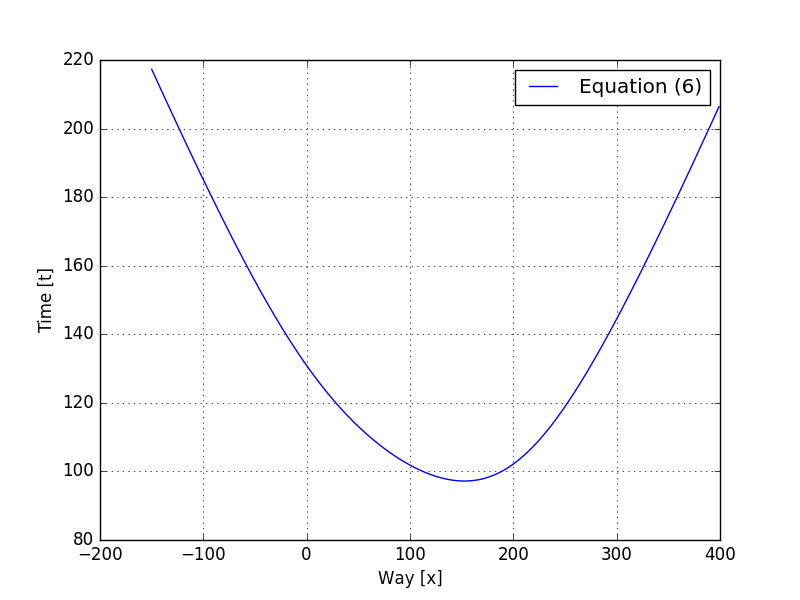
\includegraphics[width=0.9\textwidth]{lifeguard_100}
    \caption{Rettungsschwimmer mit $m=100$}\label{lifeguard_100}
\end{figure}

Aus Abbildung~\ref{lifeguard_100} ist ersichtlich, an welcher Stelle $x$ optimal sein wird. Wie wir rechnersch bereits bewiesen haben, ist diese Extremalstelle, hier ein globales Minimum, die kürzeste mögliche Zeit, die der Retter zurücklegen wird. Wir haben nun die Lösung mathematisch mit der Gleichsetzung der 1. Ableitung zu 0 erhalten. 


\subsection{Versicherungsprämienrechner}
Eine Versicherung will herausfinden bei welcher Prämie ihr Gewinn maximal ist. Der Durchschnittliche Schadensbetrag der Kunden liegt bei CHF 103. Interpoliert man die zur Verfügung gestellten Daten erhält man folgende Graphen.
\begin{figure}[!ht]
    \centering
    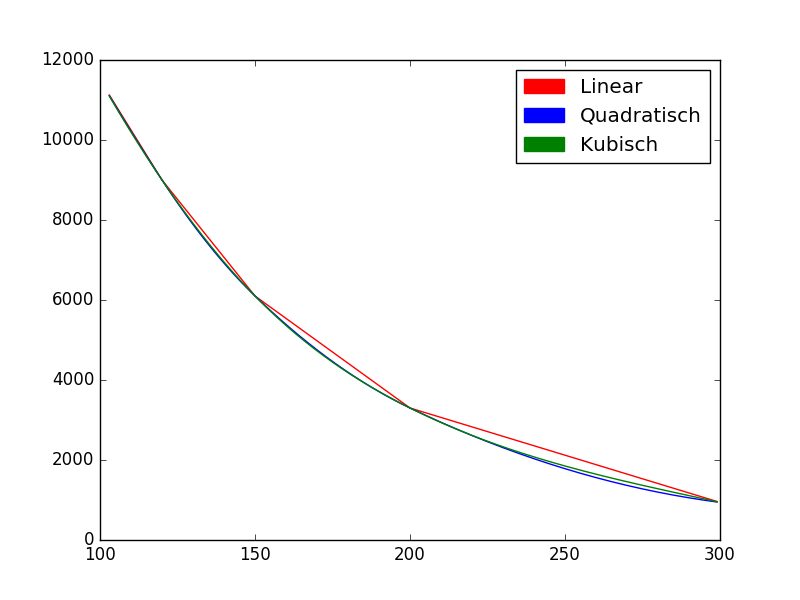
\includegraphics[width=0.9\textwidth]{customres}
    \caption{Kunden im Bezug auf Prämien}\label{customers}
\end{figure}
Die Unterschiede zeigen sich durch Art der Interpolation. Es wurden eine Lineare, eine Quadratische und schlussendlich noch eine kubische Interpolation gemacht. \\
Nun muss der Gesamtgewinn berechnet werden. Die Formel dafür ist schnell gefunden: $Gewinn = Pr\ddot{a}mie * Kunden - Schaden*Kunden$ Diese Formel sagt aleine sehr wenig aus. Der entscheidende Faktor hierbei ist die Anzahl Kunden, welche wir noch haben bei einer Prämie. Also ist die Funktion um die Kunden im verhältnis zur prämie herauszufinden um einiges relevanter für diesen Anwendungsfall.
Je nach verwendeter Interpolationsart erhält man verschiedene Resultate: \\
\begin{itemize}
    \item Linear: Bei einer Prämie von CHF 181 wird ein Gewinn von CHF 340'392 erwirtschaftet.
    \item Quadratisch: Bei einer Prämie von CHF 184 wird ein Gewinn von CHF 323'214 erwirtschaftet.
    \item Kubisch: Bei einer Prämie von CHF 187 wird ein Gewinn von CHF 323'051 erwirtschaftet.
\end{itemize}
Den Unterschied in den Prämien und dem Profit kann in diesem Grafen gut erkannt werden.
\begin{figure}[!ht]
    \centering
    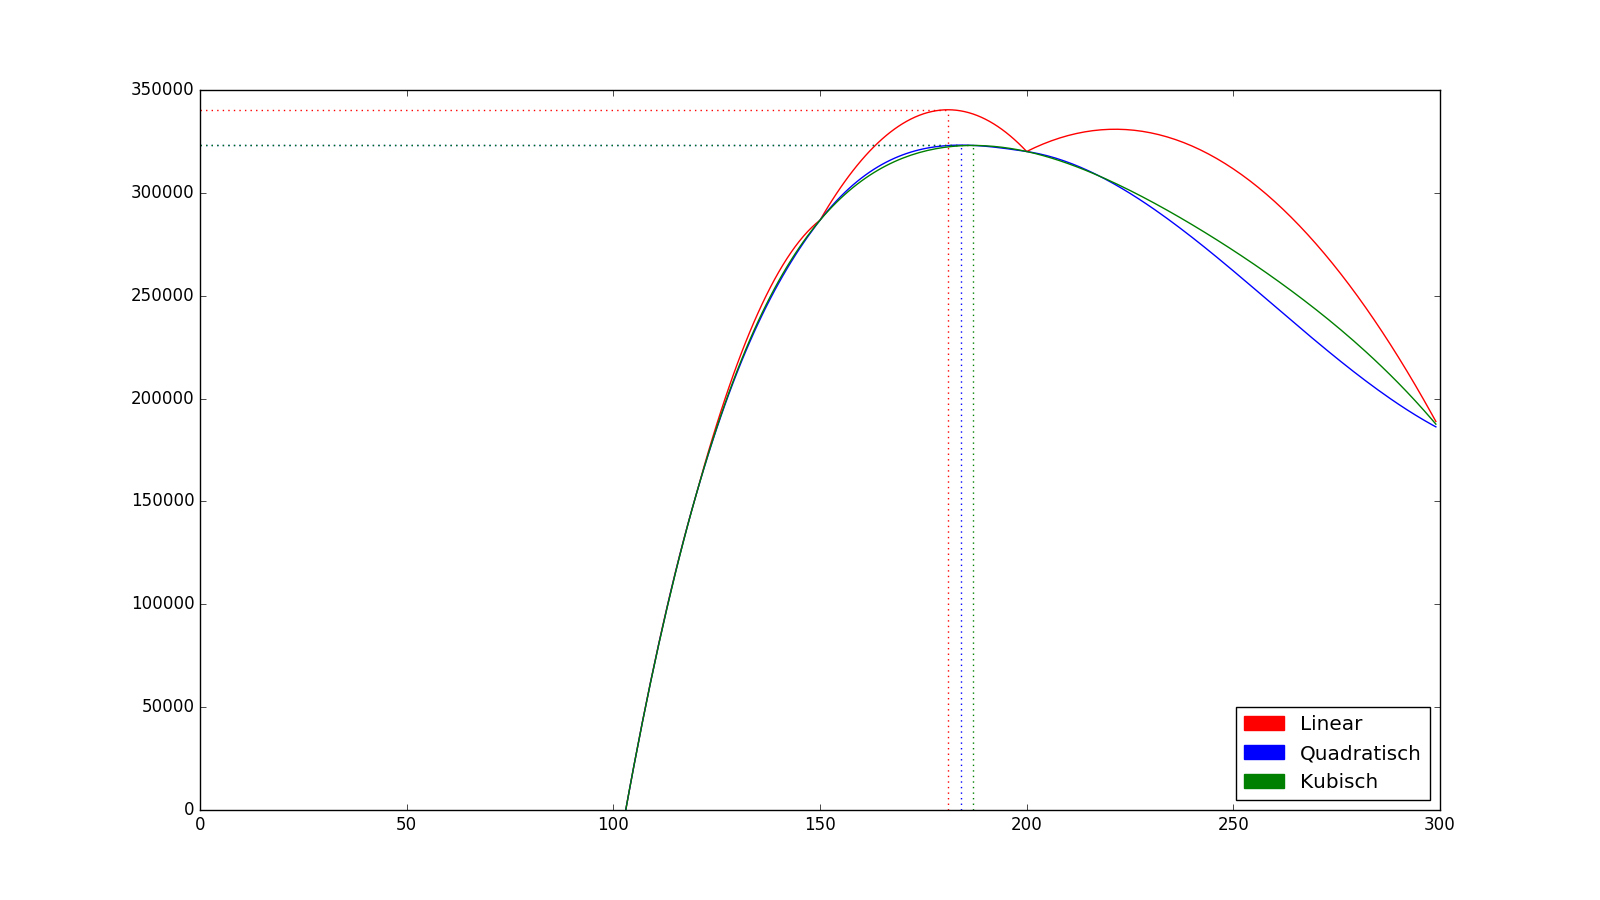
\includegraphics[width=0.9\textwidth]{profit}
    \caption{Der Gesamtgewinn}\label{fig:figure1}
\end{figure}
Mann erkennt, das die lineare Interpolation zu einigen Ecken in der Kurve führt, was hier sicher nicht das gewünschte Resultat ist, ausser wenn diese ein spezifisches Ereigniss darstellen (zum Beispiel man wird teurer als eine andere Versicherung.) Da dies hier wahrscheinlich nicht der Fall ist, kann die Lineare Version meiner meinung nach ignoriert werden. Der Unterschied zwischen der quadratischen und kubischen Implementation bei der Prämie, welche den höchsten Gewinn erziehlt liegt bei CHF 3 und kann ebenfalls ignoriert werden.
\subsubsection{Diskussion des Resultats} % (fold)
\label{ssub:diskussion_des_resultats}
Das erhaltene Resultat funktioniert aus meiner Sicht nur für eine Versicherung möglich, welche ein Monopol auf dem Gebiet hat, in welchem Sie agiert. Dies ist klar erkennbar daran, dass die Kunden im verhältnis zur Prämie eine schöne Funktion bilden. Bei einer Versicherung mit Konkurenz sollten eigentlich Einbrüche erkennbar sein, wenn man Teurer als eine andere Versicherung wird und diese über den selben Umfang verfügt. \\
Generell ist es nicht gut die Prämie generell über alle Kunden zu mitteln. Schon alleine durch den Fahrzeug wert kann ein riesiger Unterschied entstechen. Ein kunde mit seinem Fünfzehn jährigen Opel wird bei einem Totalschaden weit weniger Kosten verursachen als ein Kunde mit einem Brandneuen Ferarri.
Ausserdem ist es eine äusserst naive Ansicht dem Kunden, welcher seit Jahren Unfallfrei fährt die selbe Prämie abzuverlangen wie der Person, welche in diesem Jahr schon zwei Unfälle hatte. Das Riskio das der Erstgenannte in diesem Jahr einen Unfall baut ist wesentlich geringer und ausserdem hat er diesen Schaden über Jahre abbezahlt.\\
Allgemein ist es ein sehr grundsätzliches Modell, welches in der Praxis so nicht verwendet werden kann.
% subsubsection diskussion_des_resultats (end)
\section{Diskussion}
\subsubsection{Anwendbarkeit der Methoden}
Alle Methoden können als Hilfestellung für die Findung von Extremalstellen verwendet werden. Durch ihre unterschiedlichen Voraussetzungen ist aber nicht jede der Methoden gleich gut für eine Problemstellung geeignet. Beim Bisektionsalgorithmus ist die Voraussetzung, dass ein Intervall bekannt ist, in welchem eine Extremalstelle liegen muss. Ausserdem muss sichergestellt sein, dass nur eine solche Stelle darin liegt. Was zunächst als massive Einschränkung aufgenommen werden kann, kann in der Realität möglicherweise sogar als Vorteil betrachet werden, sofern die Punkte im Kontext einfach bestimmt werden können.\\
Ähnlich wie der Bisektionsalgorithmus verhält sich das Gradientenverfahren. Bei dieser Methode ist vorausgsetzt, dass ein Punkt bekannt ist, welcher links von einer Extremalstelle liegt. Der Algorithmus könnte für eine bestimmte Anwendung so erweitert werden, dass ein Punkt gewählt wird, welcher über eine gefundene Extremalstelle hinaus weitersucht. Dort sieht sich aber die Gefahr, dass der nächste Punkt viel weiter weg sein könnte, was eine höhere Laufzeit zur Folge hätte.\\
Beim Nelder-Mead Algorithmus sehen wir den Vorteil, dass wir ausser zwei frei wählbare Zahlen nichts benötigen, um eine Extremalstelle zu bestimmen.
\subsubsection{Vorteile/Nachteile}
Für die Gegenüberstellung von Vor- und Nachteilen der einzelnen Algorithmen muss deutlich hervorgehoben werden, dass der Anwendungsbereich bestimmt, welcher Algorithmus sich am Besten eignet. Generell kann man sagen, dass der Nelder-Mead Algorithmus dank den wenigen zu erfüllenden Vorbedingungen wohl als beste Lösung abschneidet. 
\subsubsection{Gegenüberstellung der Laufzeiten}
Einen direkten Vergleich der Laufzeiten an sich ist heikel. Wir können aus den obigen Diskussionen entnehmen, dass beim einfachen Gradientenverfahren ein Zeitverlust akzeptiert werden muss, falls der Startpunkt sich sehr weit von der Extremalstelle weg befindet. Anders als das Bisektions- und Gradientenverfahren verwendet der Nelder-Mead Algorithmus die 1. Ableitung nicht. Dies führt zu einem Zeitgewinn, welchen wir nicht direkt gemessen haben, aber trotzdem erahne lässt, dass dies ein Vorteil verschafft.

\section{Referenzen}
\begin{list}{}{}
\item $^1$ http://www.b-landau.de/simplex-algorithmus/
\end{list}

\pagebreak
\section{Anhang}

\lstset{language=Python,
        breaklines=true,
        basicstyle=\ttfamily\small,
        keywordstyle=\color{keywords},
        commentstyle=\color{comments},
        stringstyle=\color{green},
        showstringspaces=false,
        identifierstyle=\color{blue},
        procnamekeys={def,class}}

\subsubsection{Hilfsklasse für Funktionshandling}
\lstinputlisting[language=Python]{../functionhelper/function.py}

\subsubsection{Gradientenverfahren}
\lstinputlisting[language=Python]{../gradientenverfahren.py}

\subsubsection{Nelder-Mead}
\lstinputlisting[language=Python]{../neldermead.py}

\subsubsection{Bisektionsverfahren}
\lstinputlisting[language=Python]{../bisection.py}

\subsubsection{Rettungsschwimmeraufgabe}
\lstinputlisting[language=Python]{../lifeguard.py}

\subsubsection{Versicherungsaufgabe}
\lstinputlisting[language=Python]{../insurance.py}

\end{document}
